\section{Presentation Logic Layer}

%What pages will be present in your project? briefly indicate how your web site will be organized

Below we define the pages we are going to develop in the BookRec application. All the pages have been developed using html or jsp.

\begin{itemize}
    \item \textbf{Starting page}: the very first page that the user sees. On this page the user can search for books, genres, or other users;
    \item \textbf{Sign-up page}: this page allows the user to register in BookRec.
    \item \textbf{Login page}: this page allows the user to log in if the user is already registered in BookRec.
    \item \textbf{Homepage}: the page seen by the user once they are logged in.
    \item \textbf{Search results}: shows a list of findings accorfing to the search.
\end{itemize}

Each page, except for the login and the starting page include and header with the logged in user information
which allows them to logout.

\subsection{Starting page}

%For the main pages put a mockup and describe it in detail.

\begin{figure}[h]
    \centering
    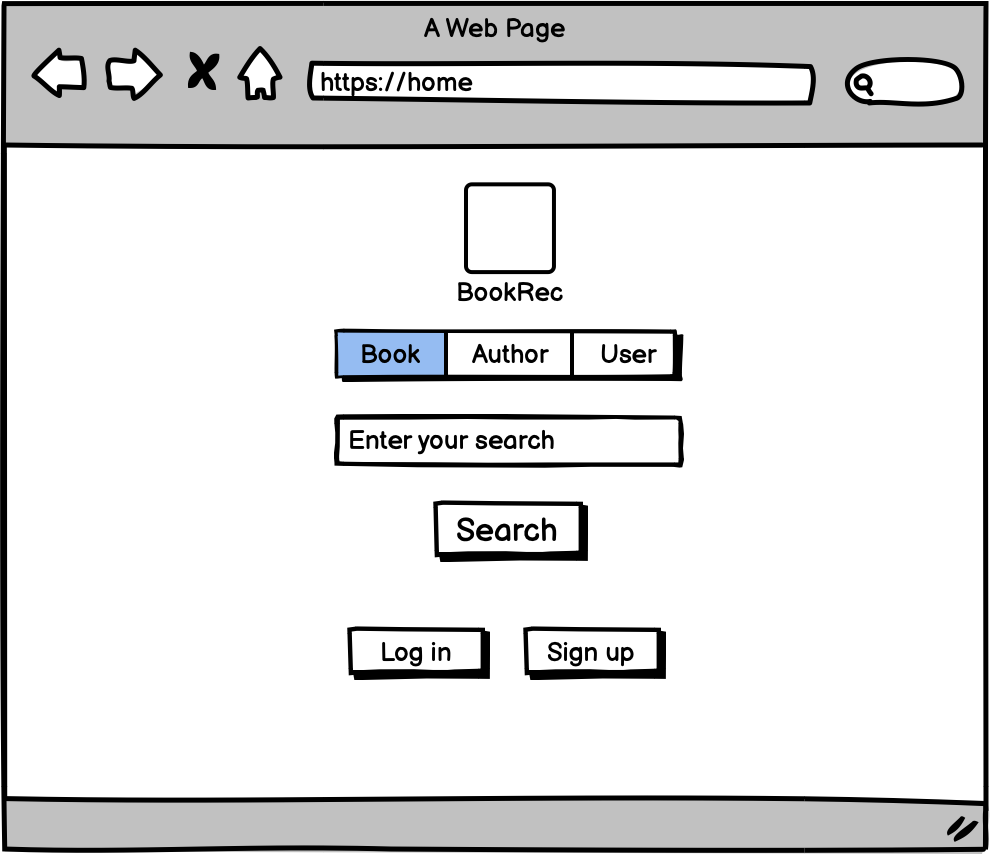
\includegraphics[width=0.5\linewidth]{sections/PLL/start.png}
    \caption{Starting page}
    \label{fig:start}
\end{figure}

Starting page is the very first page that the user sees. On this page the user can search for books, genres, or other users

\subsection{Sign up page (Interface mockup)}

\begin{figure}[h]
    \centering
    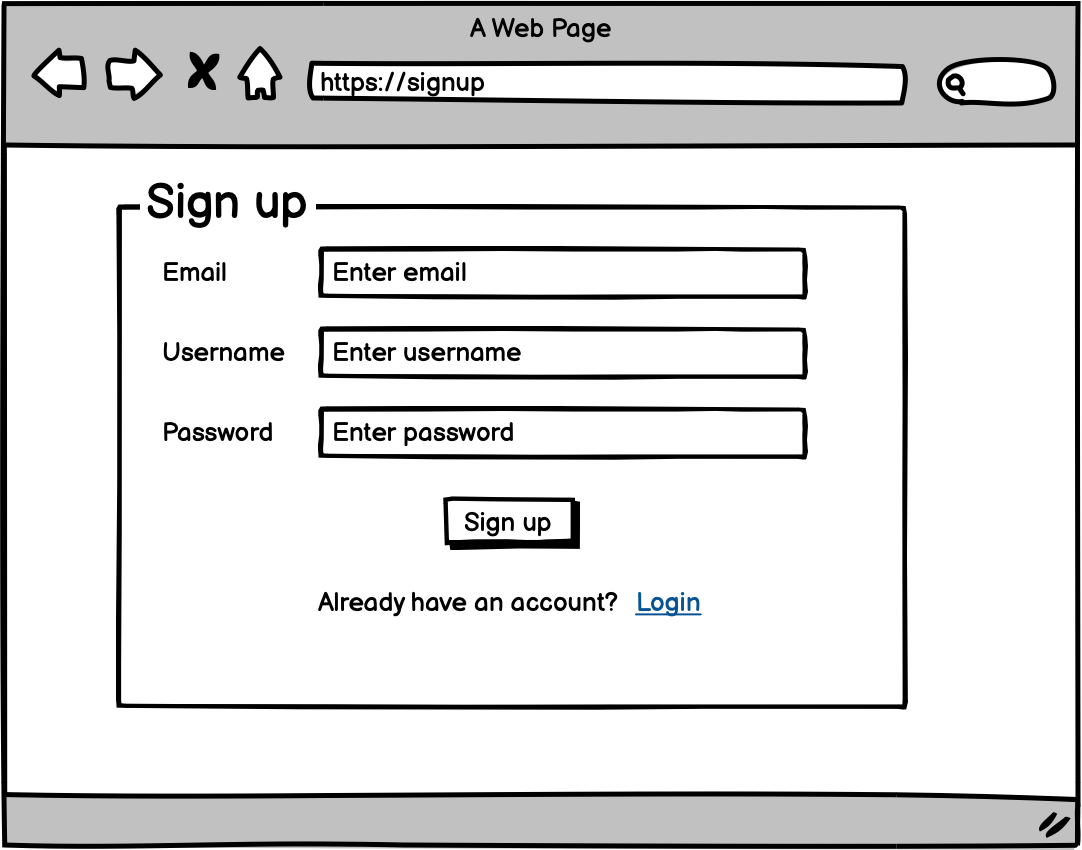
\includegraphics[width=0.5\linewidth]{sections/PLL/signup.png}
    \caption{Sign up page}
    \label{fig:signup}
\end{figure}

In Figure \ref{fig:signup} we described a simple sign up page. On the Sign up page, the user can provide their credentials to use to access their account. The information a user must provide is the email, the password, and the username. The password to be provided must contain at least 8 characters, at least one number, and at least one upper case letter. After clicking on Sign up the user's credentials are added their credentials to the database, and they are redirected to the homepage. If the credentials do not comply with those required, an error message is returned. If a user already has an account, they can proceed to the login page.

\subsection{Login page (Interface mockup)}

\begin{figure}[h]
    \centering
    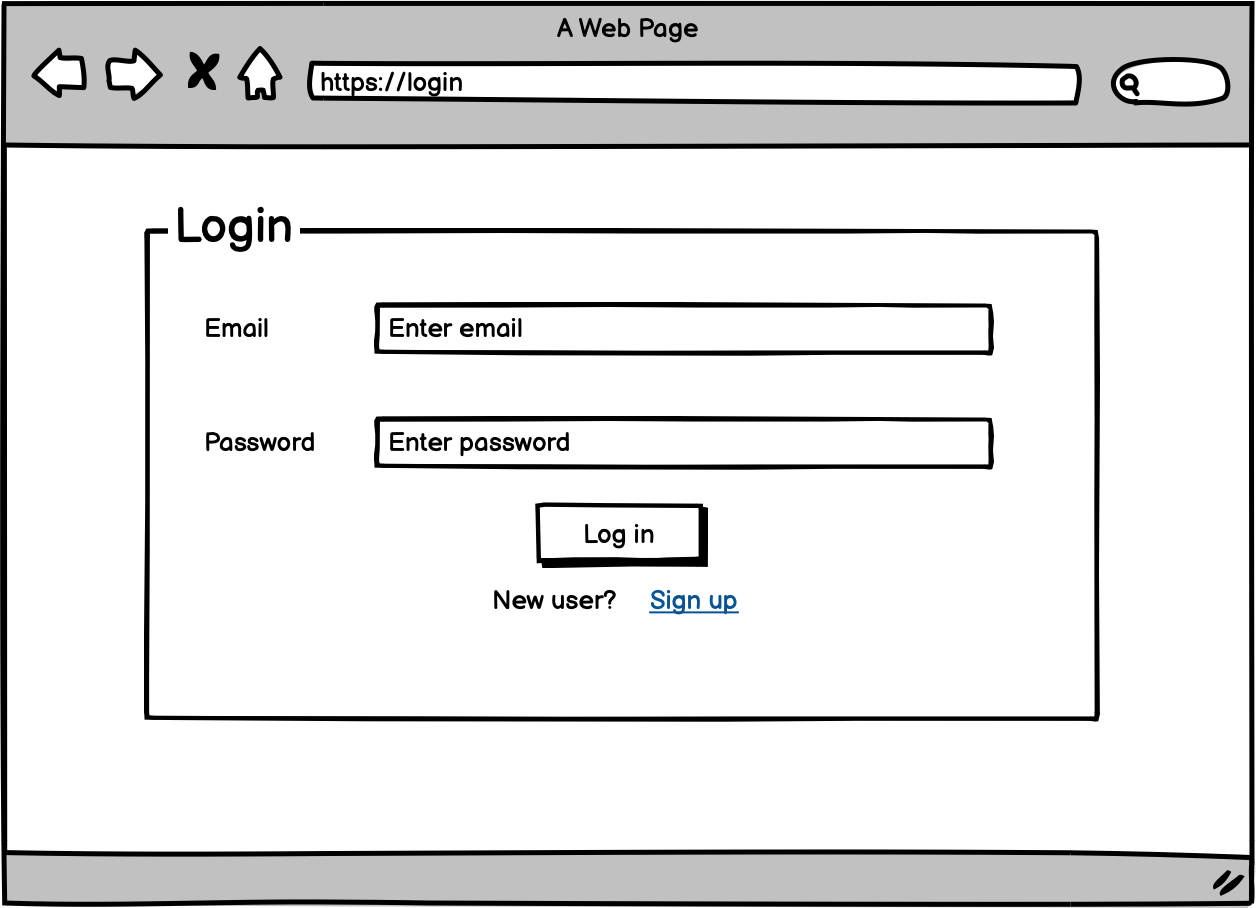
\includegraphics[width=0.5\linewidth]{sections/PLL/Login.png}
    \caption{Login page}
    \label{fig:login}
\end{figure}

The login form in Figure \ref{fig:login} is similar to the sign up page. If a user is not registered, they can proceed to the sign up page. To enter the system a user must provide their email and password that they entered when signing up.

\subsection{Search results (Interface mockup)}

\begin{figure}[h]
    \centering
    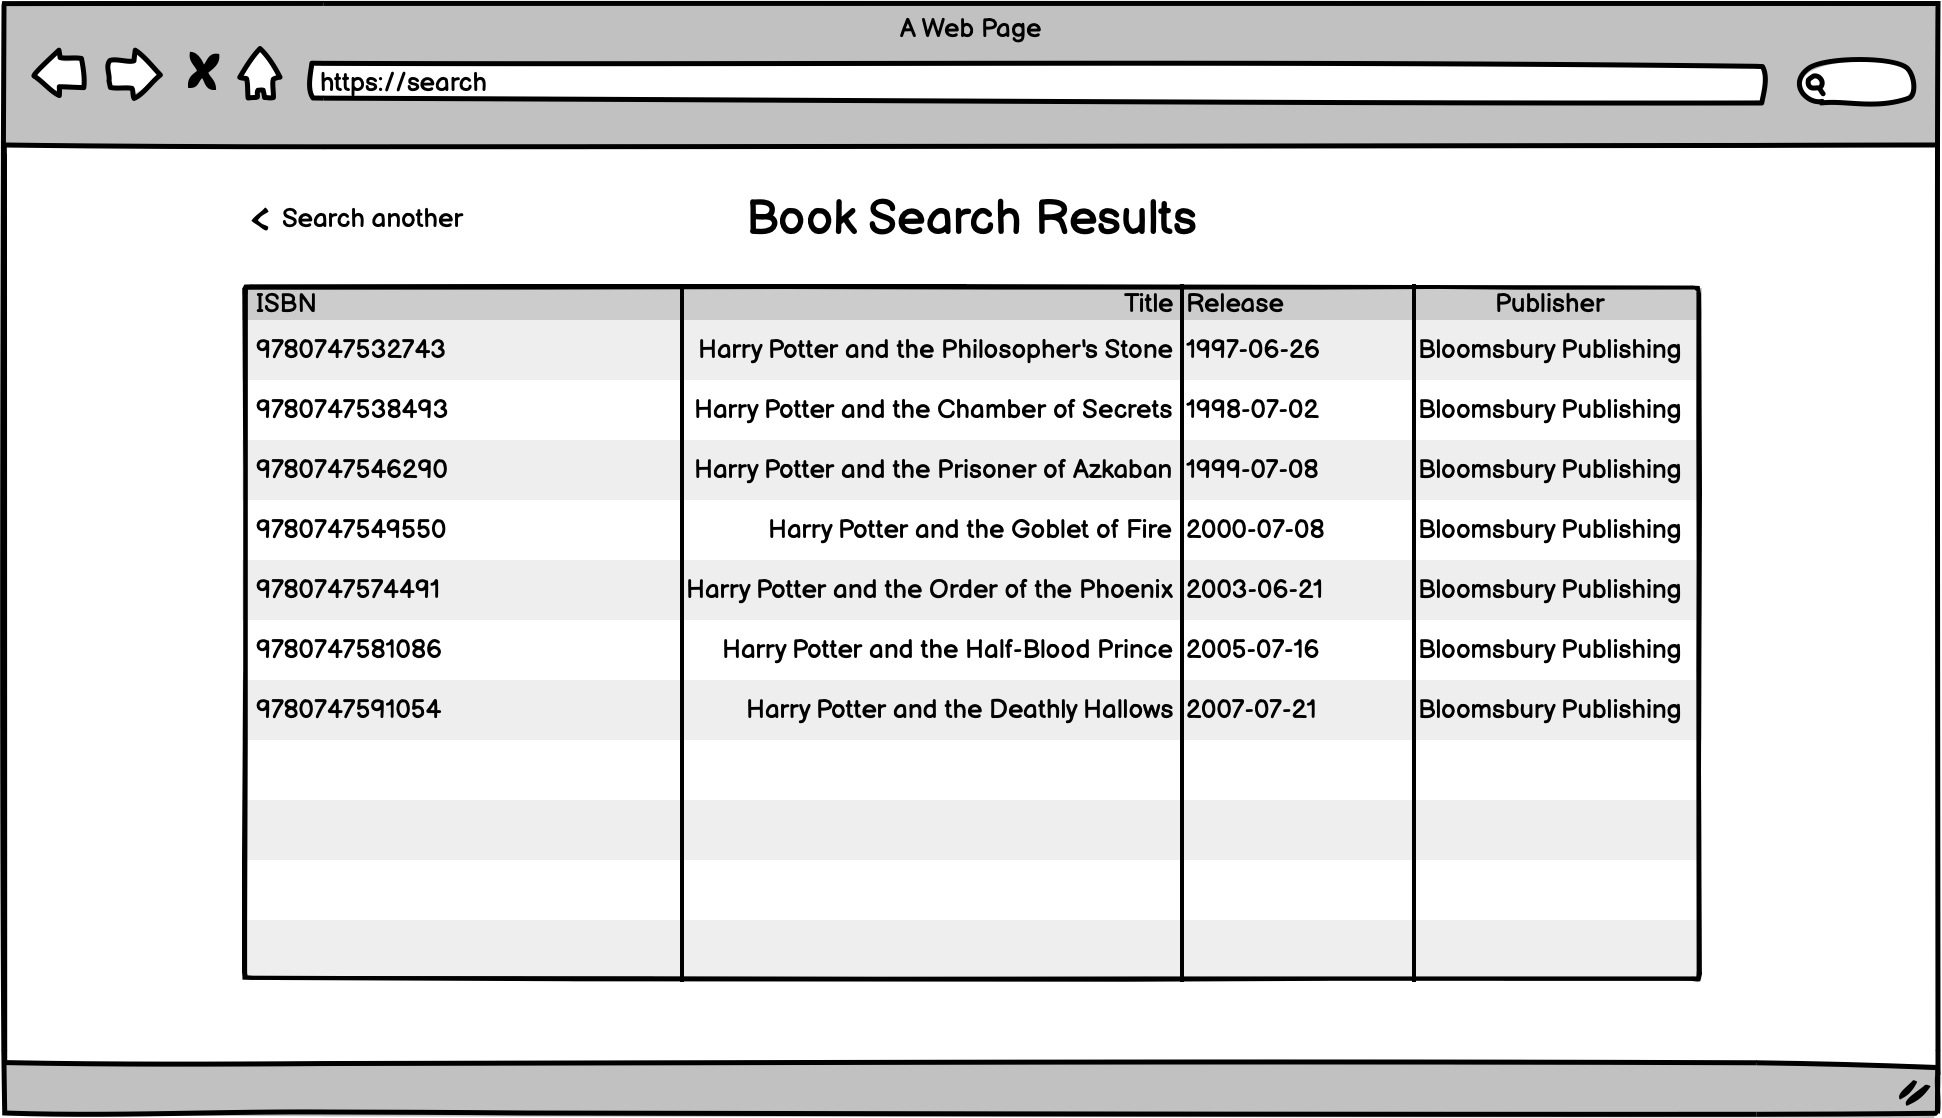
\includegraphics[width=0.6\linewidth]{sections/PLL/search-book.png}
    \caption{Search book results page}
    \label{fig:search-book}
\end{figure}

The search page in Figure \ref{fig:search-book} displays a table of results for a book search. The table contains the following information: ISBN number, name, release date, and the publisher of the book. If there are no matches in the database, "No matches found" message will be displayed. User can navigate back to search for another book, author or user.

\begin{figure}[h]
    \centering
    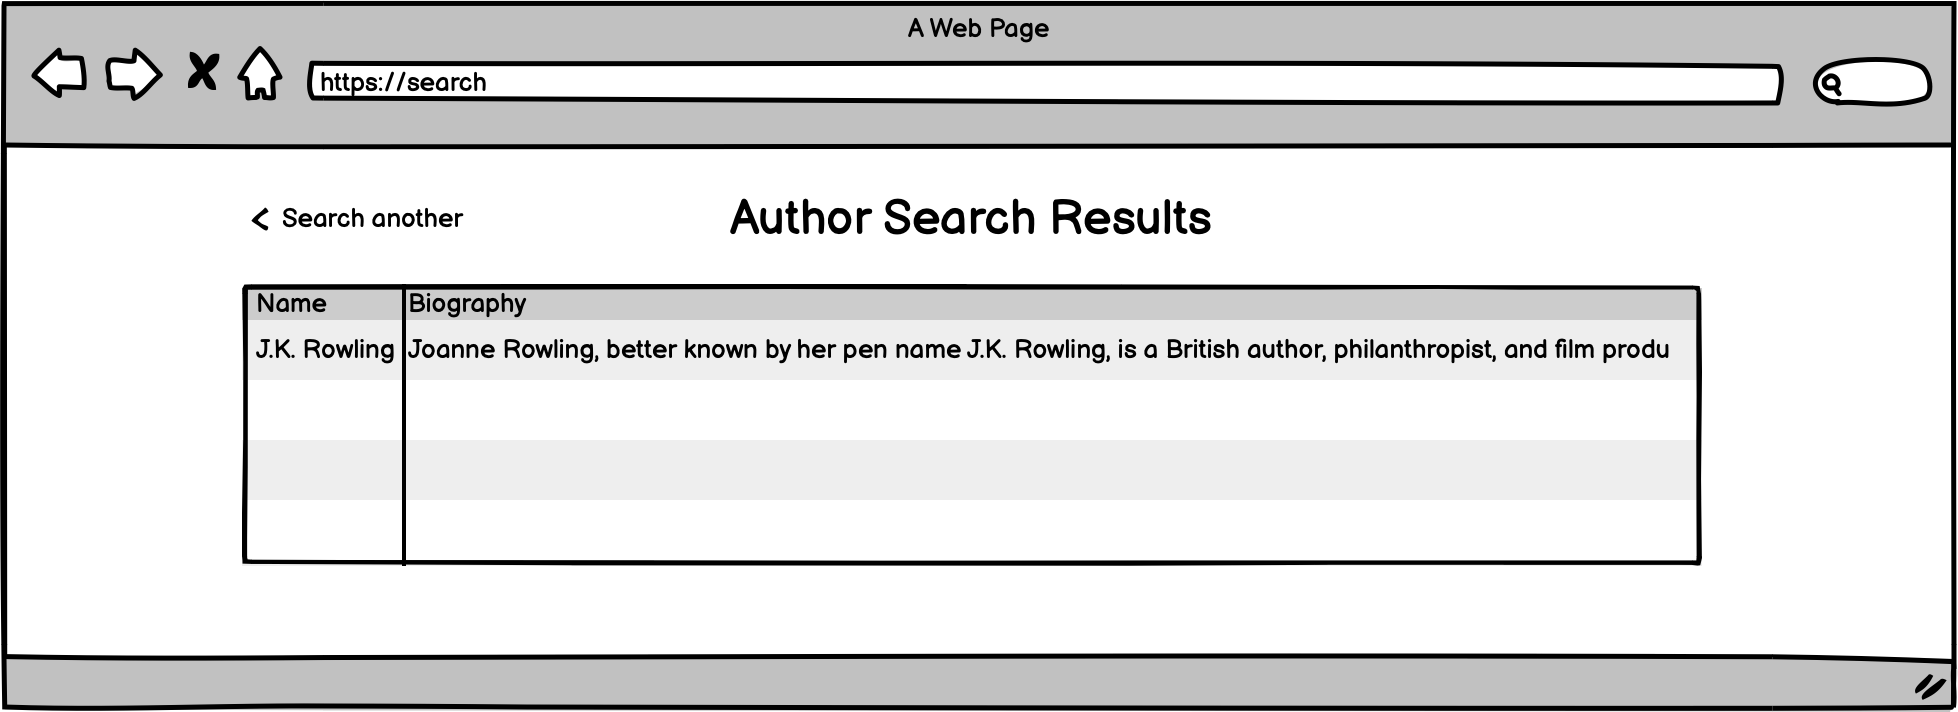
\includegraphics[width=0.6\linewidth]{sections/PLL/search-author.png}
    \caption{Search author results page}
    \label{fig:search-author}
\end{figure}

The search form in Figure \ref{fig:search-author} displays a table of results for author search. The table contains the name of the author and their biography. If there no authors are matched in the database, "No matches found" message will be displayed. The user search is similar, the table of user search will display a table of matched users, so that the user can explore other users' recommendations by navigating to their profiles.